\chapter{Requirements und Use Cases}\label{ch:requirements-und-use-cases}


\section{Systemebene}\label{sec:systemebene}

%% Die Anforderungen aus der Aufgabenstellung sind nicht vollständig. Die Struktur der nachfolgenden Kapitel soll Sie bei der Strukturierung der Analyse unterstützen. Dokumentieren Sie die Ergebnisse der Analysen entsprechend.

\subsection{Stakeholder}\label{subsec:stakeholder}

%% Ermitteln Sie die Stakeholder für das Projekt und listen Sie diese hier auf.

\paragraph{Externe Stakeholder}
\begin{itemize}
    \item Auftraggeber
    \begin{itemize}
        \item Erfüllung aller spezifizierten Anforderungen
        \item Pünktliche Lieferung zum vorgegebenen Termin
        \item Verwendung der vorgegebenen Hard- und Software
    \end{itemize}
    \item Betreuer
    \begin{itemize}
        \item Erreichen der Ziele am Ende jeder Phase
        \item Möglichst vollständige Dokumentation als Rückmeldungsgrundlage
    \end{itemize}
    \item Benutzer
    \begin{itemize}
        \item System stellt keine Gefahr dar
        \item Information über Fehlerzustände
        \item Möglichst selten Eingreifen erforderlich
        \item Hoher Durchsatz
        \item Einfache Bedienung und Inbetriebnahme (Dokumentation)
    \end{itemize}
    \item Verwaltung TI-Labor
    \begin{itemize}
        \item Keine Beschädigung der Anlagen
    \end{itemize}
\end{itemize}

\paragraph{Interne Stakeholder}
\begin{itemize}
    \item Entwickler
    \begin{itemize}
        \item Gute Testbarkeit
        \item Einfache Erweiterbarkeit und Modularität
        \item Einheitliche Schnittstellen und Benennungen
        \item Dokumentation (im Code) für Fehlersuche und Teamarbeit
    \end{itemize}
\end{itemize}

\subsection{Anforderungen}\label{subsec:anforderungen2}

%% In der Aufgabenstellung sind Anforderungen an das System gestellt.
%% Arbeiten Sie diese hier auf und ergänzen Sie diese entsprechend der Absprachen mit dem Betreuer.
%% Achten Sie auf die entsprechende Atribuierung.
%% Berücksichtigen Sie auch mögliche Fehlbedienungen und Fehlverhalten des Systems.

\subsection{Systemkontext}\label{subsec:systemkontext2}

\begin{figure}
    \centering
    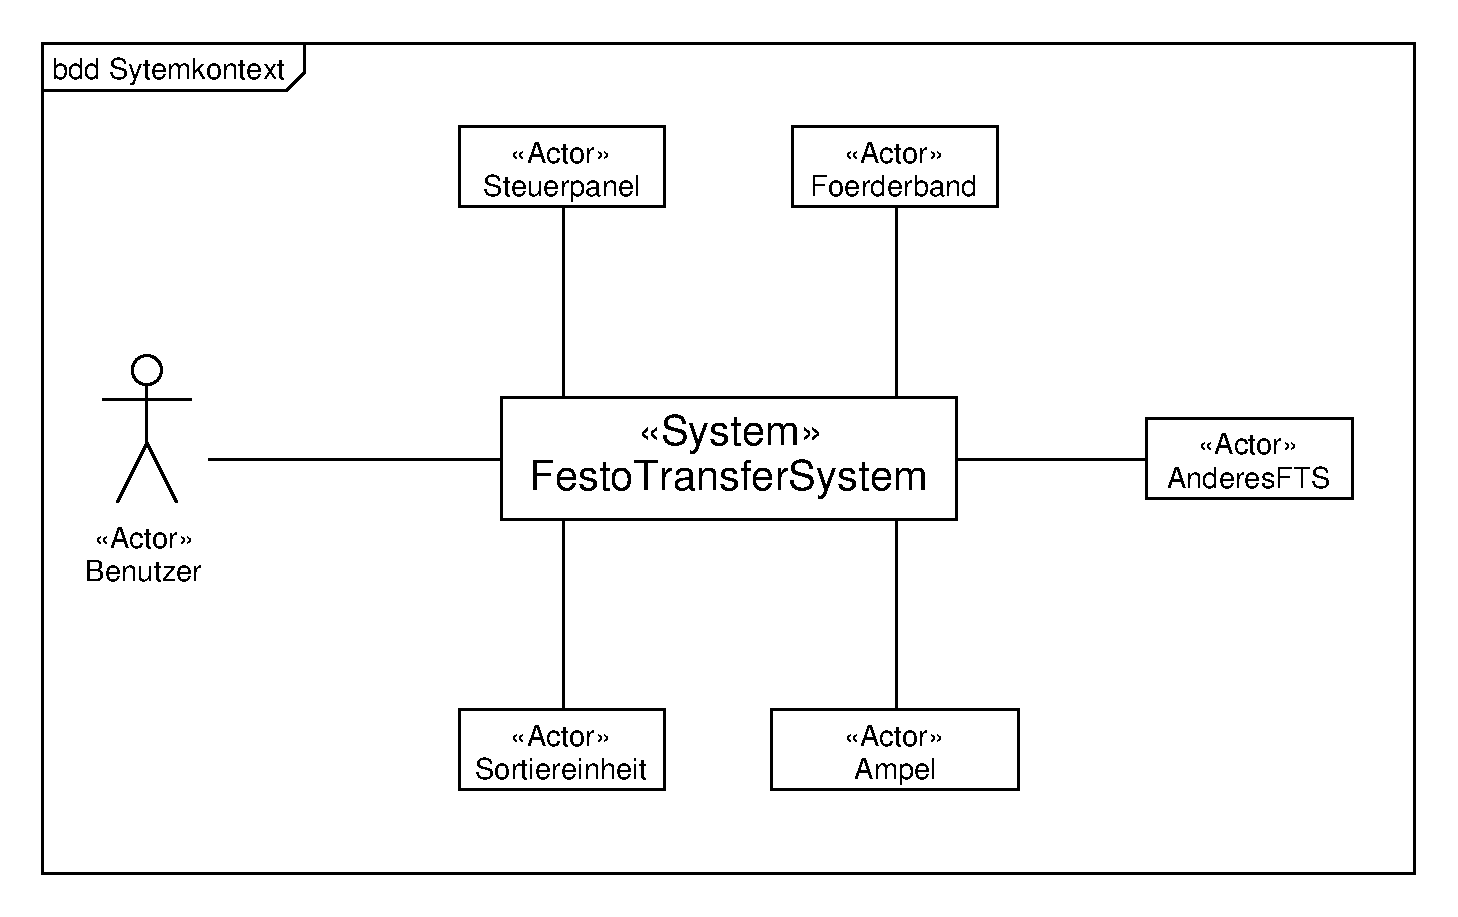
\includegraphics[width=\textwidth]{../out/diagrams/stage1/systemkontext.pdf}
    \caption{Systemkontext}
    \label{fig:systemkontext}
\end{figure}


Betrachte Abbildung \ref{fig:systemkontext}.
Die Systemsicht bringt umliegende Aktorik des Systemkontext und System selber miteinander in Beziehung.

\paragraph{Akteure}

\begin{itemize}
    \item Control\_Panel\\
    Steuerungspanel der Anlage.
    Sie stellt einen START-, STOP- und RESET-Button zur Verfügung.

    \item Conveyor\_Belt\\
    Auf Förderband werden Werkstücke durch das System bewegt.
    \item FTS\_2\\
    Die jeweils andere Förderanlage, mit der das System kommuniziert.
    \item E\_Stop\\
    Ein Button zum Auslösen des Emergency-Stops.
    \item Metal\_Detector\\
    Metall-Sensor zum Erfassen des Materials eines Werkstückes.
    \item Height\_Measurement\\
    Höhen-Sensor zum Erfassen des Materials eines Werkstückes.
    \item Stoplight\\
    Ampel, die durch verschiedene LED-Einstellungen Zustandsinformationen der Anlage anzeigt.
    \item Sorting\_Mechanism\\
    Das System besitzt allgemein einen Aussortier-Mechanismus.
    Dieser ist in einer von zwei Varianten in die Anlage eingebaut:
    \begin{itemize}
        \item Ejector\\
        Ein Auswerfer, der sich bei Stromzufluss ausfährt und so Werkstücke in die Rampe stoßen soll.
        Ohne Strom ist der Aussortiermechanismus offen.
        \item Switch\\
        Eine Weiche, die sich bei Stromzufluss öffnet und Werkstücke durchlässt.
        Ohne Strom ist der Aussortiermechanismus geschlossen und befördert Werkstücke langsam in die Rampe.
    \end{itemize}
    \item LightBarrier\\
    Das System besitzt diverse Lichtschranken als Trigger und zur Steuerung des Kontrollflusses
    \begin{itemize}
        \item LightBarrier\_Start\\
        Lichtschranke am Anfang eines Förderbandes.
        Die Unterbrechung dieser Lichtschranke setzt das Förderband in Bewegung.
        \item LightBarrier\_Ramp\\
        Lichtschranke an der Rampe, in der die Werkstücke aussortiert werden.
        Die kurze Unterbrechung dieser Lichtschranke kann als erfolgreiche Aussortierung interpretiert werden.
        Eine stetige Unterbrechung signalisiert eine volle Rutsche.
        \item LightBarrier\_Height\\
        Lichtschranke an der Position des Höhensensors.
        Die Unterbrechung dieser Lichtschranke startet eine Höhenmessung.
        \item LightBarrier\_Switch\\
        Lichtschranke vor dem Aussortiermechanismus der Anlage.
        Die Unterbrechung startet den Aussortieralgorithmus.
        \item LightBarrier\_End\\
        Lichtschranke am Ende eines Förderbandes.
        Die Unterbrechung dieser Lichtschranke kann das transferieren des Werkstückes an die nächste Anlage einleiten.
        Am Ende der zweiten Anlage werden bei Unterbrechung dieser Lichtschranke Werkstück-Informationen an der Konsole ausgegeben.
    \end{itemize}
\end{itemize}

%% Use Cases werden aus einer bestimmten Sicht erstellt.
%% Dokumentieren Sie diese mittels Kontextdiagramm oder Use Case Diagramm.
%% Die Use Cases und Test Cases müssen zu der hier verwendeten Nomenklatur konsistent sein.

\subsection{Use Cases / User Stories}\label{subsec:use-cases-user-stories}

%% Dokumentieren Sie hier, welche Use Cases/ User Stories Sie auf der Systemebene implementieren müssen.
%% Die Test Cases sollen später zu den Use Cases/ User Stories konsistent sein.

%% < Hier kommt die genaue Beschreibung der Use.
%% Pro Anforderung eine Tabelle benutzen. Die Tabelle nach Belieben vervielfältigen. >

\begin{usecase}{1}{UseCase Name}{hoch}
\addCollum{Mainflow}{
\item[1)] do something
\item[2)] do this
\item[2a)] or tihs
}\addCollum{Alternate flow}{
\item[1)] do something
\item[2)] do this
\begin{itemize}
    \item[1)] Very long text: Lorem ipsum dolor sit amet, consectetur adipiscing elit,
    \item[2)] do this
\end{itemize}
\item[2a)] or tihs
}
\end{usecase}
\addTextCollum{Description}{
    Lorem ipsum dolor sit amet, consectetur adipiscing elit,
    sed do eiusmod tempor incididunt ut labore et dolore magna aliqua.
    Ut enim ad minim veniam, quis nostrud exercitation ullamco laboris
    nisi ut aliquip ex ea commodo consequat. Duis aute irure dolor in
    reprehenderit in voluptate velit esse cillum dolore eu fugiat nulla pariatur.
    Excepteur sint occaecat cupidatat non proident, sunt in culpa qui officia
    deserunt mollit anim id est laborum
}

% eine referenz zu einem UC sieht so aus:
siehe  \nameref{uc:1}.


\section{Systemanalyse}\label{sec:systemanalyse}

%% Ihr technisches System hat aus Sicht der Software bestimmte Eigenschaften.
%% Was muss man für die Entwicklung der Software in Struktur, Schnittstellen,
%% Verhalten und an Besonderheiten wissen?
%% Wählen Sie eine Kapitelstruktur, die am besten zur Dokumentation Ihrer Ergebnisse geeignet ist.


\section{Softwareebene}\label{sec:softwareebene}

%% Sie sollen Software für die Steuerung des technischen Systems erstellen.
%% Aus den Anforderungen auf der Systemebene und der Systemanalyse ergeben sich
%% Anforderungen für Ihre Software.
%% Insbesondere wird sich die Software der beiden Anlagenteile in einigen Punkten unterscheiden.
%% Dokumentieren Sie hier die Anforderungen, die sich speziell für die Software ergeben haben.

\subsection{Systemkontext}\label{subsec:systemkontext}

%% Wie sieht der Kontext Ihrer Software aus? Wie erfolgt die Kommunikation mit Nachbarsystemen?
%% Liste der ein- und ausgehenden Signale/Nachrichten.

\subsection{Anforderungen}\label{subsec:anforderungen}

%% Welche wesentlichen Anforderungen ergeben sich aus den Systemanforderungen für Ihre Software?
%% Berücksichtigen Sie auch mögliche Fehlbedienungen und Fehlverhalten des Systems.

